%qepaper.tex
\documentclass[12pt,letterpaper]{article}
\usepackage{mathptmx}
\usepackage[margin=1in]{geometry}

\usepackage{tabularx, longtable, pdflscape, adjustbox}  % for 'tabularx' environment and 'X' column type
\usepackage{ragged2e}  % for '\RaggedRight' macro (allows hyphenation)
\newcolumntype{Y}{>{\RaggedRight\arraybackslash}X} 
\usepackage{booktabs}  % for \toprule, \midrule, and \bottomrule macros 

\usepackage{setspace}
%\onehalfspacing
\doublespacing
%\singlespacing

\usepackage{amssymb,latexsym}
\usepackage[round,sort]{natbib}
\usepackage{fancyhdr}
\usepackage{lastpage}
\usepackage{graphicx,multirow}
\graphicspath{ {qepaper/} }

% Bold Table and Figure captions
\usepackage{caption}
\captionsetup{figurename=FIGURE}
\captionsetup{tablename=TABLE}
\captionsetup[figure]{labelfont=bf}
\captionsetup[table]{labelfont=bf}

% Turns off all section numbering
\setcounter{secnumdepth}{0} 

\usepackage{titling}

  % Places all tables at end of document and creates AOM-style table-here placeholders
  \usepackage[nolists]{endfloat} % Places all figures and charts at end of manuscript and adds 'insert table x about here' lines.
  \renewcommand{\figureplace}{
    \begin{center}
    \begin{singlespace}
    ------------------------------------\\
    Insert \figurename \ \thepostfig\ about here.\\
    ------------------------------------
    \end{singlespace}
    \end{center}}
  \renewcommand{\tableplace}{%
    \begin{center}
    \begin{singlespace}
    ------------------------------------\\
    Insert \tablename \ \theposttbl\ about here.\\
    ------------------------------------
    \end{singlespace}
    \end{center}}

  \usepackage{titlesec}
   \titleformat{\title}
       {\filcenter\normalfont\bfseries\uppercase}{\thetitle}{1em}{}
  \titleformat{\section}
    {\filcenter\normalfont\bfseries\uppercase}{\thesection}{1em}{}
  \titleformat{\subsection}
    {\normalfont\bfseries}{\thesubsection}{1em}{}
  \titleformat{\subsubsection}[runin]
   {\normalfont\bfseries\slshape}{\thesubsubsection}{1em}{\hspace*{\parindent}}
       
\usepackage{tabu}
\usepackage{textcomp}
\usepackage{listings}
\usepackage{hyperref}
\usepackage{verbatim}
\usepackage{tabu}
\hypersetup{
    colorlinks=true,
    linkcolor=blue,
    filecolor=cyan,      
    urlcolor=cyan,
    citecolor=blue,
}

\usepackage{etoolbox}

\makeatletter

% Patch case where name and year are separated by aysep
\patchcmd{\NAT@citex}
  {\@citea\NAT@hyper@{%
     \NAT@nmfmt{\NAT@nm}%
     \hyper@natlinkbreak{\NAT@aysep\NAT@spacechar}{\@citeb\@extra@b@citeb}%
     \NAT@date}}
  {\@citea\NAT@nmfmt{\NAT@nm}%
   \NAT@aysep\NAT@spacechar\NAT@hyper@{\NAT@date}}{}{}

% Patch case where name and year are separated by opening bracket
\patchcmd{\NAT@citex}
  {\@citea\NAT@hyper@{%
     \NAT@nmfmt{\NAT@nm}%
     \hyper@natlinkbreak{\NAT@spacechar\NAT@@open\if*#1*\else#1\NAT@spacechar\fi}%
       {\@citeb\@extra@b@citeb}%
     \NAT@date}}
  {\@citea\NAT@nmfmt{\NAT@nm}%
   \NAT@spacechar\NAT@@open\if*#1*\else#1\NAT@spacechar\fi\NAT@hyper@{\NAT@date}}
  {}{}

\lstset{
basicstyle=\ttfamily,
columns=flexible,
breaklines=true
}
\newenvironment{hypothesis}{
  	\itshape
  	\leftskip=\parindent \rightskip=\parindent
  	\noindent\ignorespaces}

\fancypagestyle{plain}{
  \renewcommand{\headrulewidth}{0pt}
  \fancyhf{}
}	

\begin{document}
\setlength{\droptitle}{-5em}
\title{\textbf{\large Heterogeneity in Knowledge Flows of Regions: Impact on Invention Quality}}
\date{\vspace{-12ex}}

\maketitle
\thispagestyle{empty}
\renewcommand{\abstractname}{\normalsize ABSTRACT}
\begin{abstract}
\normalsize
\noindent Using patent citations as measures of knowledge flows, we explore if the different types of knowledge flows in a region affect the quality of inventions originating in that region. We leverage a database of worldwide urban centers  obtained from remote sensing data and find that  local knowledge flows  do not seem to impact the inventive quality of regions. However, knowledge flows within the firm across regions seem to have a positive effect on invention quality.
\end{abstract}

\newpage
\pagestyle{fancy}
\fancyhf{}
\lhead{Heterogeneity in Knowledge Flows of Regions: Impact on Invention Quality}
\rhead{\thepage}

%\section*{Introduction}
\cite{Burt1992} and \cite{Winter1995} and \cite{Clark2008}
\begin{itemize}
\item Suggest that invention quality is of key interest to strategy scholars as it has been known to affect firm outcomes. It must be clear that you are talking to strategy scholars looking at geographical implications for firm innovation strategy.

\item Review the literature around the antecedents of invention quality and suggest that implications of knowledge spillovers on invention quality have not been examined. At this point it should be clear to you what indeed has been examined.

\item List all the various antecedents of invention quality discussed in the literature, and suggest that there is a conflicting message in how local knowledge flows and MNC parent-subsidiary flows should help. The hypotheses do not have to be about all the four quadrants, but for just one. And your paper can serve the purpose of opening up a research agenda as well as addressing a specific question (are there precedents of this?).

\item Suggest that it is important for us to look for things that a firm can control that may have an effect on invention quality (this is after you have demonstrated that invention quality leads to better firm outcomes), and that while there may be many factors that do influence firm outcomes, that they may not also lend themselves easily for firms to change. Identify the few that firms can do something about and suggest that determining the nature of geographic collaboration/building up of is one such deliberate strategy.

\item Discuss the literature from economic geography and the stylized fact that knowledge should have an impact. 

\item Suggest an alternate literature that casts doubt on the above stylized fact.

\item Lead into the research question about how it is unclear what effect local knowledge spillovers should have vis-a-vis MNC/subsidiary and other potential factors. Be crystal clear that all you intend to understand is what the net effect of the two opposing effects may be.

\item patent citations are only the tools, so while you should bring this up, it should be only to claim legitimacy for this method and draw on prior work that though not without controversy, patent citations have been used as a measure of knowledge flows. And any conclusions that you will draw from this study will have to be limited to the extent that this is as evidenced by patent citations. For robustness you could do  applicant cited patents, examiner cited patents, and applicant+examiner cited patents. As well as the time period wise, with a 5 year window to receive citations (prior work has used this)
\end{itemize}

Scholars of economics and strategy have for long recognized that clusters and agglomeration economies play an important role in fostering innovation \citep{Marshall1890, Porter1990}. Agglomeration economies arise due to labor pooling advantages, economies of specialization of local suppliers, and knowledge spillovers \citep{Porter1990, Krugman1991a}. In this study, we\footnote{This paper is the outcome of the joint work by Sai Yayavaram and me. While the changes since the version submitted to the Strategic Management Society 2017 Conference (this version has also provided with the current paper for reference) are my own, I have used the plural ``we'' throughout this paper to preserve continuity with the previous version and compatibility with future versions that was/going to be jointly authored.} examine how the nature of knowledge spillovers or flows in a region affect the quality of the inventions generated in the region.\par
Several studies have used patent citations to demonstrate that knowledge flows are localized \citep*{Jaffe1993, Almeida1999, Alcacer2006a}. Regions, however vary in their inventive output \citep*{Agrawal2014b} and the nature of knowledge flows in a region may be one source of this variation within regions. In this study we use citation data of patents applied for between 2001 and 2012 to empirically estimate the relationship between knowledge flows of a region and quality of inventions from that region. \par
The rest of the paper is organized as follows. The next section defines a framework to classify knowledge flows in a region and motivates our work by demonstrating how different regions fare differently in terms of knowledge flows. We then describe our data and methods in the following section. Our preliminary results are then presented, followed by a discussion of the results. We conclude with next steps and open questions for further research.

\section*{Theory and Hypotheses}
\subsection*{Effects of knowledge flows on quality of inventions}
\begin{itemize}
\item Justify why the 2x2 classification is appropriate. Discuss the four quadrants in more detail, say by including examples and statistics
\end{itemize}

We categorize all knowledge flows incorporated into an invention along two dimensions:  first, whether the knowledge flows among inventors are local to a geographical region or not, and second, whether knowledge flows are within the boundary of the firm or not. This classification allows us to analyze knowledge flows in four mutually exclusive, but collectively exhaustive categories as illustrated in Figure~\ref{fig:2x2}. We next describe each quadrant and discuss how the category of knowledge flow in that quadrant can affect invention quality. Within the context of this framework, we ask what is the net effect of each category of knowledge flow on invention quality, and which category of flow has the largest effect on invention quality. \par
\begin{figure}[h!]
\begin{centering}
  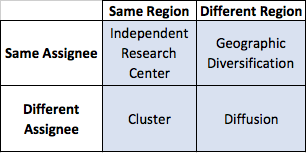
\includegraphics[width=0.4\textwidth]{2x2}
  \caption{Categories of knowledge flows}
  \label{fig:2x2}
\end{centering}
\end{figure}



The top left quadrant, labelled an ``Independent Research Center" captures those knowledge flows that reflect competence building. Since these knowledge flows  are both within the region and within the firm, these flows represent local search on two dimensions (within firm and within region).  Thus, while the competence that is being built up by the Independent Research Center can be expected to have a positive effect on invention quality, the localness of the search on both dimensions may have a negative effect on invention quality. Figure~\ref{fig:SMSSameRegionSameAssigneeFlows} depicts the knowledge flows for this category (percentage of backward citations from this region that are to the same firm or assignee and same region) across time for five regions: Bangalore, Beijing, Tel Aviv-Yafo, Boston and San Jose (core of ``Silicon Valley"). While our empirical analysis covers all the major regions of the world, we chose these five regions as illustrative examples. We note that both San Jose and Boston report a higher proportion of knowledge flows within the same firm in the same region, while Bangalore and Tel Aviv-Yafo have the lowest proportion (fewer than 1\%) of their citations from the same firm within the same region. \par

\begin{figure}[h]
\begin{centering}
  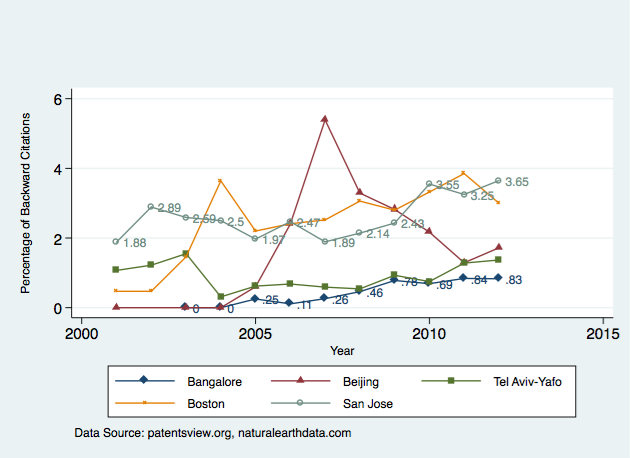
\includegraphics[width=0.90\textwidth]{SMSSameRegionSameAssigneeFlows}
  \caption{Knowledge flows within regions and within assignees}
  \label{fig:SMSSameRegionSameAssigneeFlows}
\end{centering}
\end{figure}

\begin{figure}[h!]
\begin{centering}
  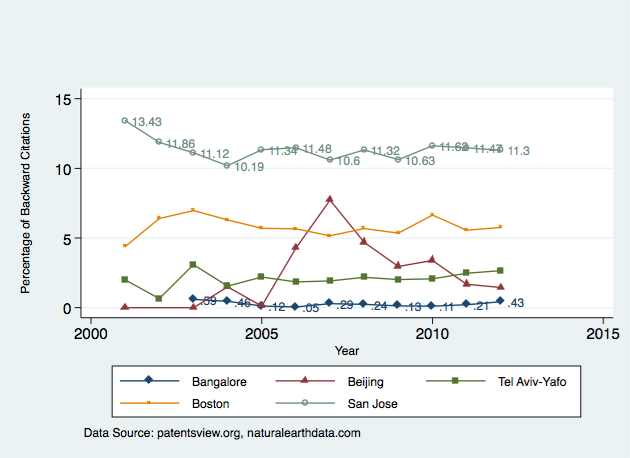
\includegraphics[width=0.90\textwidth]{SMSSameRegionDiffAssigneeFlows}
  \caption{Knowledge flows within regions and across assignees}
  \label{fig:SMSSameRegionDiffAssigneeFlows}
\end{centering}
\end{figure}
The quadrant on the bottom left, labelled ``Cluster" captures knowledge spillovers within a region. Here firms may be seen as performing local search on one dimension (within regions) but not the other (within firms). Figure~\ref{fig:SMSSameRegionDiffAssigneeFlows} depicts the knowledge flows for this category across time for the same five regions. San Jose clearly stands out from the rest, suggesting a higher amount of across firm flows of knowledge in Silicon Valley, a result consistent with several prior studies. \par
\begin{figure}[h!]
\begin{centering}
  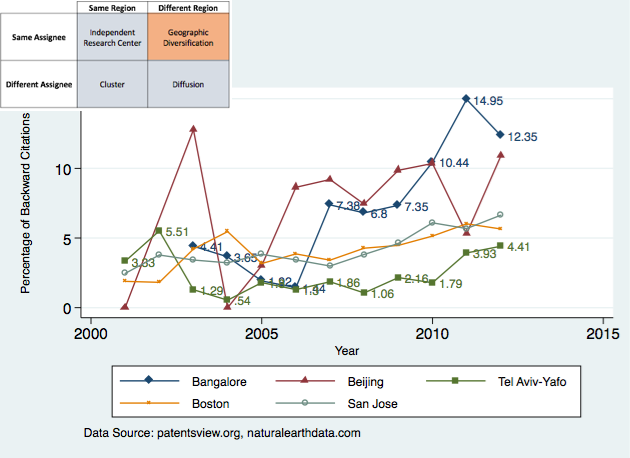
\includegraphics[width=0.90\textwidth]{SMSDiffRegionSameAssigneeFlows}
  \caption{Knowledge flows across regions and within assignees}
  \label{fig:SMSDiffRegionSameAssigneeFlows}
\end{centering}
\end{figure}

The quadrant on the top right, labelled as ``Geographic Diversification" captures local search on the dimension of the firm (across geographies) but not across regions. Innovations that are built on knowledge from several regions can be expected to benefit from the diversity of knowledge across regions. Yet, as in the previous quadrant, there is localness along the dimension of firm and such localness can have a negative effect on invention quality \citep{Rosenkopf2001}. Figure~\ref{fig:SMSDiffRegionSameAssigneeFlows} depicts the  knowledge flows for this category across time for the five regions. We note that Bangalore and Beijing have a relatively higher proportion of knowledge flows from same assignees in different locations, thus confirming the role of these regions as R\&D outposts of multinational firms.\par

\begin{figure}[h!]
\begin{centering}
  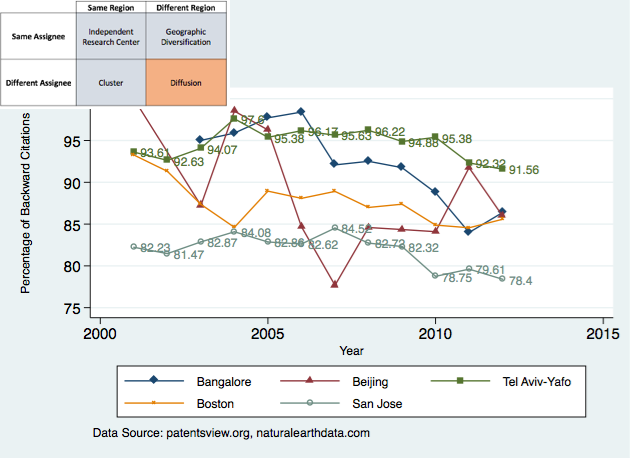
\includegraphics[width=0.90\textwidth]{SMSDiffRegionDiffAssigneeFlows}
  \caption{Knowledge flows across regions and across assignees}
  \label{fig:SMSDiffRegionDiffAssigneeFlows}
\end{centering}
\end{figure}

Finally, the bottom right quadrant labelled ``Diffusion" captures high exploration along both dimensions, indicating the development of a global pipeline \citep*{Bathelt2004}. Figure~\ref{fig:SMSDiffRegionDiffAssigneeFlows} depicts the  knowledge flows for this category across time for the five regions. We note that Bangalore, Beijing and Tel Avis-Yafo have a higher level of knowledge flows from other firms in other regions compared to Boston and San Jose, which is to be expected given that the absolute level of innovative activity in these emerging hotspots is still lower compared to that in Boston and San Jose. \par

As can be seen from the preceding discussion, prior theory suggests both positive and negative effects for each of these four categories of knowledge flows and it is not clear what the net effect will be on invention quality. This also suggests that prior theory does not provide guidance on which category of knowledge flows will have the highest effect on invention quality.  Since theory does not provide us with an answer, we rely on empirical analysis to inform us on the net effect of each category of knowledge flow on invention quality and which category has the highest effect on invention quality. \par


\subsubsection{Creating sustainable competitive advantages}
Organization learning literature suggests that specialized knowledge is routinized over time. As the dependence on FSHC reduces due to routinization of knowledge and the associated causal ambiguity arising out of tacit knowledge, the appropriability of rents by highly knowledgable workers reduces. Therefore managers intending to increase rents from exploration may chose a strategy where the rents from innovation are appropriated by highly skilled workers in the short run, but rents accrue to the firm as knowledge present in highly knowledgable workers is transformed into organizational routines. This leads me to my first hypothesis.\\

\begin{hypothesis}
{Hypothesis 1: Long term rent generating capacity of firms from exploration is characterized by an increase in costs due to appropriation by highly knowledgable employees initially, and a decrease in such costs later.
\\}
\end{hypothesis}

\subsubsection{Improving operational performance}
Given a certain organizational strategy (exploration or exploitation), the main lever by which managers may improve firm profits is by reducing costs due to appropriation by highly knowledgable workers. Managers intending to improve short term operational performance may do by reducing the extent of FSHC employed in the firm. This leads me to my second hypothesis.\\

\begin{hypothesis}
{Hypothesis 2: Given a certain organizational learning strategy for a firm, the short term profit performance in firms varies inversely with the extent of FSHC employed in the firm\\}
\end{hypothesis}

\section*{Research Design}
Fill out text here

%\scriptsize
\singlespacing
\begin{center}
\begin{table}[htbp]\centering \caption{Correlation Table\label{corrtable}}
\begin{adjustbox}{angle=90}
\begin{tabular}{l  c  c  c  c  c  c  c  c  c  c }

\hline
\multicolumn{1}{c}{Variables} &1&2&3&4&5&6&7&8&9&10\\ \hline
1. Citations Received&1.00\\
2. Non-Self Citations Received&0.99&1.00\\
3. Self Citations Received&0.68&0.60&1.00\\
4. Share Citations Made[Same Region, Same Assignee]&0.04&0.03&0.06&1.00\\
5. Share Citations Made[Same Region, Different Assignee]&0.13&0.12&0.13&0.09&1.00\\
6. Share Citations Made[Different Region, Same Assignee]&-0.01&-0.02&0.00&0.14&-0.03&1.00\\
7. Share Citations Made[Different Region, Different Assignee]&0.06&0.06&0.05&-0.10&-0.03&-0.12&1.00\\
8. Log(Total Citations Made)&0.16&0.13&0.27&0.08&0.10&0.08&0.09&1.00\\
9. Log (Num Patents)&0.31&0.29&0.26&0.12&0.18&0.03&0.21&0.68&1.00\\
10. Log (Patent Pool Size)&0.27&0.25&0.23&0.14&0.19&0.02&0.09&0.69&0.86&1.00\\ \hline
\end{tabular}
\end{adjustbox}
\end{table}
\end{center}


\begin{table}[htbp]\centering \caption{Summary Statistics \label{sumstat}}
\begin{tabular}{l c c  c}\hline\hline
\multicolumn{1}{c}{\textbf{Variable}} & \textbf{Mean}
 & \textbf{Std. Dev.} & \textbf{N}\\ \hline
Citations Received & 241.719 & 2063.915  & 57456\\
Non-Self Citations Received & 123.856 & 1147.495  & 57456\\
Self Citations Received & 36.581 & 360.104  & 57456\\
Share Citations Made[Same Region, Same Assignee] & 0.042 & 0.087  & 24324\\
Share Citations Made[Same Region, Different Assignee] & 0.015 & 0.05  & 24324\\
Share Citations Made[Different Region, Same Assignee] & 0.069 & 0.119  & 24324\\
Share Citations Made[Different Region, Different Assignee] & 0.444 & 0.258  & 24324\\
Log (Total Citations Made) & 3.55 & 2.237  & 24324\\
Log (Num Patents) & 2.263 & 1.94  & 57456\\
Log (Patent Pool Size) & 4.59 & 2.373  & 54716\\
\hline
\end{tabular}
\end{table}


\normalsize
\doublespacing

\begin{itemize}
\item correlation table
\item descriptive statistics - region wise, country wise, technology class wise, time wise
\item fixed and random effects, hussman
\item tests for endogeneity
\item table with variable names and descriptions and definitions (see \cite{Funk2014})
\item add generous footnotes
\item diagram for the hypothesised relationships
\end{itemize}
\section*{Data and Methods}

We use patent citations data from the U.S. Patent Office (USPTO) as provided by patentsview.org. The USPTO provides information on assignee, the location of inventors, and year of patent application. We use this information to identify which patents belong to which region in a given year. Since there can be more than one inventor on a patent, a patent can belong to more than one region. We compare the assignee and inventor location of each patent with each assignee and inventor of each backward citation  to identify the category of knowledge flow (e.g., same assignee, different location) indicated by the backward citation. Additionally, to map location data of inventors from USPTO to regions, we use urban centers data for worldwide locations from \href{http://www.naturalearthdata.com/downloads/10m-cultural-vectors/}{Natural Earth Data} that uses remote sensing data to determine urban agglomerations (a process developed in \citet*{Schneider2003}).  While it has been common practice to use Metropolitan Statistical Areas (MSA) for analyses related to economic geography in the U.S., an equivalent measure is unavailable for the rest of the world. For comparability and consistency, we choose to use the urban centers definitions from \href{http://www.naturalearthdata.com/downloads/10m-cultural-vectors/}{Natural Earth Data} for all regions both within U.S. and outside U.S. \par
Our unit of analysis is the region-year. To be consistent with our objective of measuring knowledge flows, we restrict ourselves to those citations categorized as \textquotesingle cited by applicant\textquotesingle \ and leave out those categorized as \textquotesingle cited by examiner\textquotesingle \ because the latter may not represent knowledge flows. This decision has the additional effect of limiting our period of analysis to citing patents applied for after the year 2000 since the data on which citations were added by examiners is available for patents from only 2001 onwards. We restrict our sample to patents applied for between 2001 - 2012, but citations received till 2015. \par
\subsection{Dependent Variable}
Our primary dependent variable is the  total count of citations received (till 2015) by patents belonging to a region-year. For robustness, we also report results for total non-self citations received as the dependent variable. 

\subsection{Independent Variables}
Our independent variables are the percentage of backward citations made to each of the four categories in our defined framework: those to a) same region, same assignee, b) same region, different assignee, c) different region, same assignee, and d) different region, same assignee. \par
\subsubsection{Percentage of backward citations made to same region and same assignee}
Write some text here. Include some mathematics here.
\subsubsection{Percentage of backward citations made to same region and different assignee}
Write some text here
\subsubsection{Percentage of backward citations made to different region and same assignee}
Write some text here
\subsubsection{Percentage of backward citations made to different region and different assignee}
Write some text here

\subsection{Control Variables}
We control for the total number of citations made in the region-year, the total number of patents in the region-year, the size of the patent pool in the region-year, as well as the percentage of patents in region-year in each technology subcategory as defined by \cite*{Hall2001a}. The patent pool is the total number of patents that belong to a region up to the previous year. It is important to control for the size of the patent pool as  regions that have a larger patent pool (such as San Jose) will have more patents that can be cited and can therefore have larger within region spillovers as compared to a region that has only a small patent pool. We include region fixed effects and year dummies in all regression models so as to control for region level and year specific effects, if any. Since our dependent variable is a count variable, we used negative binomial regression analysis with fixed effects. \par

\section*{Model Estimation}
Some text followed by mathematical formula estimated

\section*{Results}
The preliminary results from our analysis are presented in Table~\ref{model123}. Model 1 reports the results for all regions worldwide, while Model 2 and Model 3 report results for U.S. locations and non-U.S. locations respectively. Across the three models we find that local knowledge flows within the firm do not seem to have a significant impact on the quality of inventions as measured by the number of citations received. This result is robust to using non-self citations as the dependent variable as presented in Table~\ref{model192021}. \par
Our preliminary findings in Table~\ref{model123} suggest no evidence that local knowledge spillovers (i.e., same region, different assignee) lead to higher quality inventions.  One possible explanation for the lack of evidence for local knowledge spillovers may be to suggest U.S. specific effects. However as the results in model 2 of Table~\ref{model123} suggest, the trend is confirmed in a U.S.-only sample. It seems therefore that the implication for the lack of effect of localized knowledge flows on invention quality is robust to regional or country sampling. \par
The effect of non-local knowledge flows however is less clear. While geographic diversification is seen to benefit all regions (Table~\ref{model123}), the effect is not statistically significant for non-U.S. locations (Table~\ref{model192021}). This may suggest that there are regional, and potentially country effects that may be able to explain the phenomenon better. Finally, building on knowledge from outside the firm and outside the region does not seem to improve invention quality.\par
\subsection{Robustness Checks}

\section*{Discussion}
Lookup other articles to determine what points need to be made here.
\subsection{On topic 1}
Text here
\subsection{On topic 2}
More text here

\section*{Limitations}
While the use of patent citations as a measure of knowledge flows has been popular in the literature, this may nevertheless be subject to error \citep*{Arora2017a}. Our definition of regions is dependent on the latitude/longitude assignment in the patentsview.org data and on the urban centers definition in the \href{http://www.naturalearthdata.com/downloads/10m-cultural-vectors/}{Natural Earth Data}. Any systematic biases in the definition of regions can create biases in measures of within region and across region knowledge flows. \par

\section*{Conclusion}
While still at a preliminary stage, our analysis seem to suggest that local knowledge flows as measured by patent citations may not have a significant effect on the quality of inventions produced in a region. This casts a doubt on the widely accepted idea that local knowledge spillovers are an important source of agglomeration economies. A potential extension of the study could be to conduct empirical analysis at the level of firm-year rather than at the region-year. We could additionally look at the additional dimension of technology (within and outside technological domain, \cite{Rosenkopf2001}) in addition to those of within/outside region and within/outside firm. This may provide us with a more nuanced understanding of the factors affecting invention quality. Future studies could potentially examine other measures of invention outcomes such as breakthrough inventions. Finally, while our work suggests that local knowledge spillovers do not affect invention quality, it is not quite as clear why this may be the case. We hope that our current work spurs further research in this direction.  

%\onehalfspacing
%\singlespacing
\renewcommand{\refname}{REFERENCES}
\bibliography{/Users/aiyenggar/code/bibliography/aiyenggar} 
\bibliographystyle{ai-amjlike}
\newpage
%\normalsize
\singlespacing
\scriptsize
{
\def\sym#1{\ifmmode^{#1}\else\(^{#1}\)\fi}
\begin{longtable}{l*{3}{c}}
\caption{Negative binomial regression analysis of invention quality (total citations received) \label{model123}}\\
\hline\hline\endfirsthead\hline\endhead\hline\endfoot\endlastfoot
                &\multicolumn{1}{c}{(1)}&\multicolumn{1}{c}{(2)}&\multicolumn{1}{c}{(3)}\\
                &\multicolumn{1}{c}{Citations}&\multicolumn{1}{c}{Citations}&\multicolumn{1}{c}{Citations}\\
                 &\multicolumn{1}{c}{Received}&\multicolumn{1}{c}{Received}&\multicolumn{1}{c}{Received}\\
\hline
Share Citations Made[Same Region, Same Assignee]&   -0.169         &   -0.104         &   -0.134         \\
                &  (0.218)         &  (0.623)         &  (0.454)         \\
Share Citations Made[Same Region, Different Assignee]&   -0.149         &   -0.191         &  -0.0919         \\
                &  (0.215)         &  (0.458)         &  (0.468)         \\
Share Citations Made[Different Region, Same Assignee]&    0.217  &    0.266  &    0.348 \\
                &  (0.012)         &  (0.037)         &  (0.004)         \\
Share Citations Made[Different Region, Different Assignee]&  0.00828         &   0.0315         &   0.0179         \\
                &  (0.789)         &  (0.499)         &  (0.661)         \\
Log (Total Citations Made)&   0.0180&   0.0198&   0.0134  \\
                &  (0.000)         &  (0.001)         &  (0.014)         \\
Log (Num Patents)&    0.785&    0.811&    0.830\\
                &  (0.000)         &  (0.000)         &  (0.000)         \\
Log (Patent Pool Size)&   -0.111&   -0.227&  -0.0944\\
                &  (0.000)         &  (0.000)         &  (0.000)         \\
\hline
Observations&9241&3885&5356         \\
Groups&1314&529&785\\
Sample&All &U.S. &Non-U.S. \\
          &Locations &Locations&Locations \\
\hline\hline
\multicolumn{4}{l}{\small \textit{p}-values in parentheses}\\
\multicolumn{4}{l}{\small All models include region fixed effects, year dummies and technology subcategory controls}\\
\end{longtable}
}

\newpage
{
\def\sym#1{\ifmmode^{#1}\else\(^{#1}\)\fi}
\begin{longtable}{l*{3}{c}}
\caption{Negative binomial regression analysis of invention quality (non-self citations received) \label{model192021}}\\
\hline\hline\endfirsthead\hline\endhead\hline\endfoot\endlastfoot
                &\multicolumn{1}{c}{(1)}&\multicolumn{1}{c}{(2)}&\multicolumn{1}{c}{(3)}\\
                &\multicolumn{1}{c}{Non-Self}&\multicolumn{1}{c}{Non-Self}&\multicolumn{1}{c}{Non-Self}\\
                &\multicolumn{1}{c}{Citations}&\multicolumn{1}{c}{Citations}&\multicolumn{1}{c}{Citations}\\
                &\multicolumn{1}{c}{Received}&\multicolumn{1}{c}{Received}&\multicolumn{1}{c}{Received}\\
\hline
Share Citations Made[Same Region, Same Assignee]&   -0.232         &   -0.183         &   -0.316         \\
                &  (0.105)         &  (0.392)         &  (0.123)         \\
Share Citations Made[Same Region, Different Assignee]&   0.0391         &   0.0945         &   0.0505         \\
                &  (0.733)         &  (0.721)         &  (0.699)         \\
Share Citations Made[Different Region, Same Assignee]&    0.195  &    0.263  &    0.174         \\
                &  (0.035)         &  (0.041)         &  (0.212)         \\
Share Citations Made[Different Region, Different Assignee]&  0.00989         &   0.0203         &  0.00983         \\
                &  (0.762)         &  (0.675)         &  (0.826)         \\
Log (Total Citations Made)&   0.0150&   0.0139  &   0.0107         \\
                &  (0.000)         &  (0.023)         &  (0.075)         \\
Log (Num Patents)&    0.772&    0.795&    0.828\\
                &  (0.000)         &  (0.000)         &  (0.000)         \\
Log (Patent Pool Size)&  -0.0453  &   -0.108 &  -0.0685  \\
                &  (0.039)         &  (0.006)         &  (0.017)         \\
\hline
Observations    &     8879         &     3732         &     5147         \\
Groups          &     1199         &      478         &      721         \\
Sample&All &U.S. &Non-U.S. \\
          &Locations &Locations&Locations \\
\hline\hline
\multicolumn{4}{l}{\small \textit{p}-values in parentheses}\\
\multicolumn{4}{l}{\small All models include region fixed effects, year dummies and technology subcategory controls}\\
\end{longtable}
}

\newpage
\begin{table}[htbp]\centering \caption{Regression Analysis of Invention Quality for Applicant \& Examiner Citations \label{ae.model123192021}}
\scriptsize
\singlespacing
\begin{tabular}{l*{6}{c}} \hline
                &\multicolumn{1}{c}{(1)}&\multicolumn{1}{c}{(2)}&\multicolumn{1}{c}{(3)}&\multicolumn{1}{c}{(4)}&\multicolumn{1}{c}{(5)}&\multicolumn{1}{c}{(6)}\\
                &\multicolumn{1}{c}{Total}&\multicolumn{1}{c}{Total}&\multicolumn{1}{c}{Total}&\multicolumn{1}{c}{Non-Self}&\multicolumn{1}{c}{Non-Self}&\multicolumn{1}{c}{Non-Self}\\
                &\multicolumn{1}{c}{Citations}&\multicolumn{1}{c}{Citations}&\multicolumn{1}{c}{Citations}&\multicolumn{1}{c}{Citations}&\multicolumn{1}{c}{Citations}&\multicolumn{1}{c}{Citations}\\
                 &\multicolumn{1}{c}{Received}&\multicolumn{1}{c}{Received}&\multicolumn{1}{c}{Received}&\multicolumn{1}{c}{Received}&\multicolumn{1}{c}{Received}&\multicolumn{1}{c}{Received}\\
\hline
Share Citations Made[Same Region, Same Assignee]&    0.211&    0.179&    0.254&    0.826&    0.899&    0.831\\
                &  (0.014)&  (0.128)&  (0.036)&  (0.000)&  (0.000)&  (0.000)\\
Share Citations Made[Same Region, Different Assignee]&   -0.393&   -0.471&  -0.0458&    0.816&    0.809&    0.811\\
                &  (0.010)&  (0.041)&  (0.808)&  (0.000)&  (0.003)&  (0.000)\\
Share Citations Made[Different Region, Same Assignee]&    0.244&    0.282&    0.326&    0.673&    0.655&    0.678\\
                &  (0.000)&  (0.002)&  (0.000)&  (0.000)&  (0.000)&  (0.000)\\
Share Citations Made[Different Region, Different Assignee]&  0.00301&   0.0243&    0.101&    0.820&    0.934&    0.802\\
                &  (0.932)&  (0.649)&  (0.036)&  (0.000)&  (0.000)&  (0.000)\\
Log (Total Citations Made)&    0.241&    0.193&    0.240&    0.180&    0.126&    0.214\\
                &  (0.000)&  (0.000)&  (0.000)&  (0.000)&  (0.000)&  (0.000)\\
Log (Num Patents)&    0.570&    0.662&    0.612&    0.634&    0.701&    0.620\\
                &  (0.000)&  (0.000)&  (0.000)&  (0.000)&  (0.000)&  (0.000)\\
Log (Patent Pool Size)&   -0.125&   -0.272&  -0.0931&  -0.0783&   -0.128&  -0.0734\\
                &  (0.000)&  (0.000)&  (0.000)&  (0.000)&  (0.000)&  (0.000)\\
Constant        &  -0.0147&    0.753&   -0.273&   -1.008&   -0.889&   -1.029\\
                &  (0.777)&  (0.000)&  (0.000)&  (0.000)&  (0.000)&  (0.000)\\
\hline
Observations    &    16111&     6449&     9662&    15701&     6324&     9377\\
Groups          &     1776&      617&     1159&     1654&      587&     1067\\
Sample&All &U.S. &Non-U.S.&All &U.S. &Non-U.S. \\
          &Locations &Locations&Locations&Locations &Locations&Locations \\
\hline\hline
\multicolumn{7}{l}{\footnotesize \textit{p}-values in parentheses}\\
\multicolumn{7}{l}{\footnotesize All regressions use negative binomial estimation on the region-year panel}\\
\multicolumn{7}{l}{\footnotesize All models include region fixed effects, year dummies and technology subcategory controls}\\
\end{tabular}
\end{table}
\end{document}
